% Templates/attributes.tex

\begin{center}
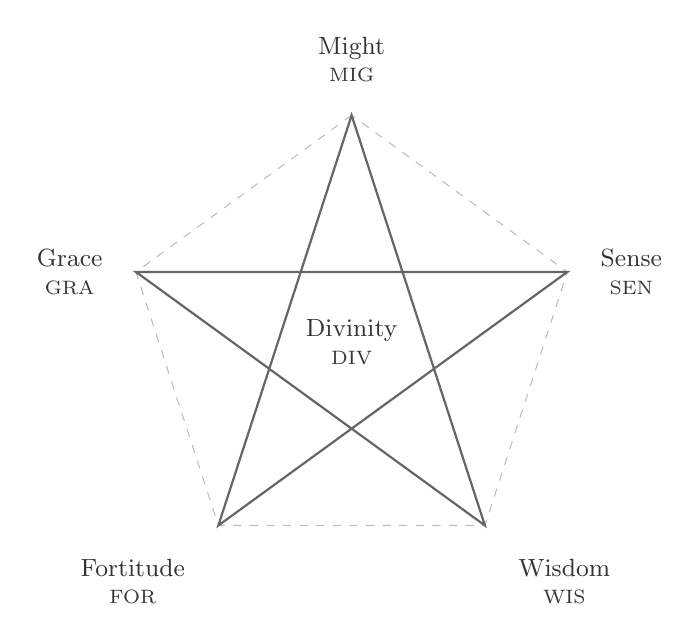
\begin{tikzpicture}[
    scale=0.9,
    % Definindo os estilos diretamente aqui para evitar o erro de "Unknown Key"
    attr_label/.style={
        font=\ringmfamily\fontsize{9}{10}\selectfont,
        text=black!80,
        align=center
    },
    attr_sigla/.style={
        font=\ringmfamily\fontsize{12}{14}\selectfont\bfseries,
        text=black
    }
]
    % Configurações de Raio
    \def\radius{3.2cm}

    % Coordenadas do Pentágono
    \foreach \i in {1,...,5} {
        \coordinate (P\i) at ({90 + (\i-1)*72}:\radius);
    }
    \coordinate (CENTER) at (0,0);

    % Desenho das Linhas de Fundo (Teia)
    \draw[lightgray, dashed] (P1) -- (P2) -- (P3) -- (P4) -- (P5) -- cycle;


    % O Pentagrama (A Estrela interna)
    \draw[thick, black!60] (P1) -- (P3) -- (P5) -- (P2) -- (P4) -- cycle;

    % Atributos nas Pontas
    % 1. MIG
    \node[attr_label, above=0.3cm] at (P1) {\ringm{Might}\\ \scriptsize MIG};
    % 2. GRA
    \node[attr_label, left=0.3cm] at (P2) {\ringm{Grace}\\ \scriptsize GRA};
    % 3. FOR
    \node[attr_label, below left=0.3cm] at (P3) {\ringm{Fortitude}\\ \scriptsize FOR};
    % 4. WIS
    \node[attr_label, below right=0.3cm] at (P4) {\ringm{Wisdom}\\ \scriptsize WIS};
    % 5. SEN
    \node[attr_label, right=0.3cm] at (P5) {\ringm{Sense}\\ \scriptsize SEN};

    \node[attr_label] at (CENTER) {\ringm{Divinity}\\ \scriptsize DIV};

\end{tikzpicture}
\end{center}